\subsection{Digital Signal Processing}
Digital Signal processing (DSP) is an engineering field focused on analyzing and altering digital signals. It takes real-world signals like voice, audio, video and then mathematically manipulates them. \cite{dsp} \par

Signals need to be processed so that the information they contain can be displayed, analyzed or converted to another type of signal. Analog-to-Digital converters take signals from the real-world and turns them into binary digital format. At this point the DSP takes over by capturing the digitized information and processes it, later to be fed back for use in the real-world. \par

\subsubsection{Sound}
\par
Sound is produced when something vibrates. The vibration causes the medium around it to vibrate as well. Vibrations in the air are called traveling longitudinal waves \cite{physics_of_sound}, which we can hear.
A sound wave is made out of two areas of high and low pressure called compressions and rarefactions (figure 3). \par

The pattern of the wave repeats after one wavelength. The height of the wave is called Amplitude. It is what determines how loud the sound will be, the greater the louder.

The wavelength and the speed of the wave determine the pitch (frequency of the sound). \par 


\begin{equation}
c = f \cdot \lambda \textnormal{, where $c=speed$, $f=frequency$, $\lambda=wavelength$}
\end{equation}

\begin{figure}[h]
	\caption[Traveling Wave]{
		Traveling wave components \cite{traveling_wave} }
	\centering
	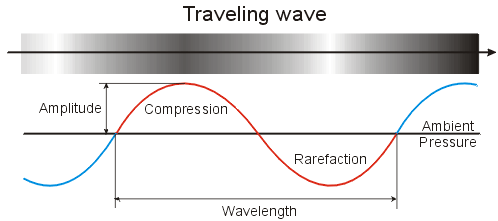
\includegraphics[width=1\textwidth, height=\textheight, keepaspectratio]{Wavelength}
\end{figure}

\subsubsection{Pitch}
In music, the pitch tells how low or high a note is. In physics, it's measured in a unit called Hertz (Hz) and it's known as frequency. A note that vibrates at 256Hz will be caused by a sound wave vibrating at 256 times/second. \par

The speed is influenced by the medium in which it travels. Under standard temperature and pressure sound's speed is 343 meters per second. \cite{speed_of_sound}

The equation (5) can be rewritten as:
\begin{equation}
f = \dfrac{c}{\lambda} \textnormal{, where $c=speed$, $f=frequency$, $\lambda=wavelength$}
\end{equation}


\subsubsection{Discrete Fourier Transformation}
The Discrete Fourier Transformation (DFT) is one of the most important operation of DSP. It is any quantity or signal that varies over time, such as the pressure of a sound wave, sampled over a finite time interval (often defined by a window function). \cite{discrete} \par

\begin{equation}
X[k] = \dfrac{1}{N} \sum_{j=0}^{N-1}(x[j] \cdot e^ {-j \cdot( \dfrac{2\pi}{N}) ) \cdot n \cdot k }  \text{ for k = 0...N-1}
\end{equation}

The DFT tells you what frequencies are present in your signal and in what proportions.
\par
It has a complexity of $O(n^2)$ so in practice the Fast Fourier Transform (FFT) algorithm is used instead. FFT runs in $O(n\cdot log(n))$

\subsubsection{Fast Fourier Transform}
Add more info about fast fourier transform

\subsubsection{Short-Term Fourier Transform}
While DFT is really good by itself, if used on an entire song it would only tell what frequencies exist, but not when they occur. This is where Short-Term Fourier Transform (STFT) comes in handy. It computes DFT over a full signal, but in small segments. Because of this we can see how frequencies change over time, which makes it a good way to compute spectrograms. (Figure 4) 

\begin{figure}[h]
	\caption[Spectrogram using Short-Term Fourier Transform]{ Spectrogram using STFT \cite{stft_fig}}
	\centering
	\includegraphics[width=1\textwidth, height=\textheight, keepaspectratio]{"resources/STFT_spectrogram"}
\end{figure}


\subsubsection{Constant-Q Transform}
In general, the transform is well suited to musical data, and this can be seen in some of its advantages compared to the fast Fourier transform. As the output of the transform is effectively amplitude/phase against log frequency, fewer frequency bins are required to cover a given range effectively, and this proves useful where frequencies span several octaves. As the range of human hearing covers approximately ten octaves from 20 Hz to around 20 kHz, this reduction in output data is significant. \cite{constant_q} \par
 See Figure 5 for a comparison between Constant-Q transform and STFT.
%work on this more


%maybe change this later
\begin{figure}[h]
	\caption[Constant Q vs STFT spectrogram of C major scale]{ Constant Q (left) vs STFT (right) spectrogram of C major scale}
	\centering
	\label{fig:cq_vs_stft}
	\includegraphics[width=1\textwidth, height=\textheight, keepaspectratio]{"resources/Q_vs_STFT"}
\end{figure}